\documentclass[10pt,letterpaper]{article}
\usepackage[latin1]{inputenc}
\usepackage{amsmath}
\usepackage{amsfonts}
\usepackage{amssymb}
\usepackage{graphicx}

\usepackage{float}
\usepackage{url}
\usepackage{hyperref}
\usepackage{ccicons}
\usepackage{svg}
\usepackage{xcolor}
\usepackage{natbib}

\topmargin -0.50in
\oddsidemargin 0.50in
\textwidth 6.0in
\textheight 9.00in
\setlength{\parindent}{0pt}

\def\uline{\underline}


\title{\em Marche Pontificale}
\author{J.L.A. Uro}
\date{23 September 2017}

%The commands to typeset this file are:
%
%\begin{verbatim}
%  latex -shell-escape foo.tex
%  latex -shell-escape foo.tex
%  dvips tunebook-sample.dvi
%  ***OR***
%  pdflatex -shell-escape foo.tex (2x; edit hyperref.cfg to del dvips)
%\end{verbatim}

% -----     


\begin{document}
	
	\maketitle
	
	\tableofcontents\label{tabofcon}
		
	\section{Introduction}
	The \textbf{\emph{Pontifical Anthem and March}} (Italian: \textit{Inno e Marcia Pontificale}), also known as the
	\textbf{\emph{Papal Anthem}}, is the \href{https://en.wikipedia.org/wiki/Honors_music}{anthem} played
	to mark the presence of the \href{https://en.wikipedia.org/wiki/Pope}{Pope} or one of his representatives,
	such as a \href{https://en.wikipedia.org/wiki/nuncio}{nuncio}, and on other solemn occasions \hyperref[ref1]{[1]}\label{ref1-a}. When
	the \href{https://en.wikipedia.org/wiki/Flag_of_Vatican_City}{Vatican's flag} is ceremonially raised,
	only the first eight \href{https://en.wikipedia.org/wiki/bar_(music)}{bars} are played \hyperref[ref2]{[2]}\label{ref2-a}. \\
	
	While the Papal Anthem also serves as the
	\href{https://en.wikipedia.org/wiki/national_anthem}{national anthem} of the \href{https://en.wikipedia.org/wiki/Holy_See}{Holy See}
	and the \href{https://en.wikipedia.org/wiki/Vatican_City}{Vatican City State}, the Vatican stresses
	that it ``is not to be understood as a national anthem"; it is a
	composition whose words and music ``speak to the heart of many
	throughout the world who see in \href{https://en.wikipedia.org/wiki/Rome}{Rome} the \href{https://en.wikipedia.org/wiki/Holy_See}{See of Peter}" \hyperref[ref1]{[1]}\label{ref1-b}.
	
	\subsection{History}
	\label{history}
	
	The music was composed in 1869 by \href{https://en.wikipedia.org/wiki/Charles_Gounod}{Charles Gounod},
	for the celebration on April 11, 1869 of \href{https://en.wikipedia.org/wiki/Pope_Pius_IX}{Pope Pius IX}'s golden jubilee of priestly ordination. The purely instrumental piece in three parts (see \hyperref[ref3]{[3]}\label{ref3-a}), originally called \textbf{\emph{Marche pontificale}} (\href{https://en.wikipedia.org/wiki/French_language}{French} for ``Pontifical March''),
	became extremely popular from its first performance \hyperref[ref1]{[1]}\label{ref1-c} \hyperref[ref2]{[2]}\label{ref2-b}.\\
	
	On October 16, 1949, \href{https://en.wikipedia.org/wiki/Pope_Pius_XII}{Pope Pius XII} declared it the
	papal anthem, replacing \href{https://en.wikipedia.org/wiki/Viktorin_Hallmayer}{Viktorin Hallmayer}'s
	\emph{\href{https://en.wikipedia.org/wiki/Marcia_Trionfale_(Hallmayer)}{Marcia trionfale}} (1857),
	which, being still the papal anthem when the Vatican City State was
	founded in 1929, had been treated also as the new state's anthem.
	Gounod's \emph{Marche Pontificale} was first performed in this new role
	during a ceremony on \href{https://en.wikipedia.org/wiki/Christmas_Eve}{Christmas Eve} of 1949, one
	day before the opening of the \href{https://en.wikipedia.org/wiki/Jubilee_(Christian)}{Holy Year}
	1950. The old anthem too was played for a last time, almost as a token
	of respect \hyperref[ref1]{[1]}\label{ref1-d}. \\
	
	At that time, \href{https://en.wikipedia.org/wiki/Antonio_Allegra}{Antonio Allegra} (1905--1969), who
	was then one of the organists of \href{https://en.wikipedia.org/wiki/St._Peter's_Basilica}{St. Peter's Basilica}, wrote \href{https://en.wikipedia.org/wiki/Italian_language}{Italian} lyrics for Gounod's music \hyperref[ref4]{[4]}\label{ref4-a}. Other lyrics have been composed for the music in various
	languages and by different authors \hyperref[ref4]{[4]}\label{ref4-b}. Some of these versions
	are not directly related to the papacy, e.g. \href{https://en.wikipedia.org/wiki/Rudy_Villanueva}{Rudy Villanueva}'s \href{https://en.wikipedia.org/wiki/Cebuano_language}{Cebuano} prayer,
	\emph{\href{https://en.wikipedia.org/wiki/Yutang_Tabonon}{Yutang Tabonon}} (``Beloved Land''), for
	protection for the \href{https://en.wikipedia.org/wiki/Philippines}{Philippine} nation. In 1991,
	\href{https://en.wikipedia.org/wiki/Raffaello_Lavagna}{Raffaello Lavagna} of \href{https://en.wikipedia.org/wiki/Savona}{Savona} (born 1918)
	wrote \href{https://en.wikipedia.org/wiki/Latin}{Latin} lyrics for a four-voice choir, on an arrangement by
	\href{https://en.wikipedia.org/wiki/Alberico_Vitalini}{Alberico Vitalini} \hyperref[ref3]{[3]}\label{ref3-b}.
	
	\subsection{Italian lyrics by \hyperref[ref4]{Allegra (1949)}\label{ref4-c}}
	\label{italian-lyrics-by-allegra-1949}
	
	\begin{minipage}{3.0in}		
\begin{description}
	%\tightlist
	\item[]
	\textbf{Original Italian}%\footnote{}\\
	\hspace*{0.333em}
	
	Roma immortale di Martiri e di Santi,
	
	Roma immortale accogli i nostri canti:
	
	Gloria nei cieli a Dio nostro Signore,
	
	Pace ai Fedeli, di Cristo nell'amore.\\
	\hspace*{0.333em}
	
	A Te veniamo, Angelico Pastore,
	
	In Te vediamo il mite Redentore,
	
	Erede Santo di vera e santa Fede;
	
	Conforto e vanto a chi combatte e crede,\\
	\hspace*{0.333em}
	
	Non prevarranno la forza ed il terrore,
	
	Ma regneranno la Verit�, l'Amore.
\end{description}
	\end{minipage}
\begin{minipage}{3.0in}
	\begin{description}
	%\tightlist
	\item[]
	\textbf{An English translation}%\footnote{}\\
	\hspace*{0.333em}
	
	O Rome immortal of Martyrs and Saints,
	
	O immortal Rome, accept our praises:
	
	Glory in the heavens to God our Lord,
	
	And peace to men who love Christ!\\
	\hspace*{0.333em}
	
	To You we come, Angelic Pastor,
	
	In You we see the gentle Redeemer,
	
	The Holy Heir of true and holy Faith;
	
	Comfort and refuge of those who believe and fight.\\
	\hspace*{0.333em}
	
	Force and terror will not prevail,
	
	But Truth and Love will reign.
\end{description}
\end{minipage}
\vfill
\begin{figure}[!h]
	\centering
	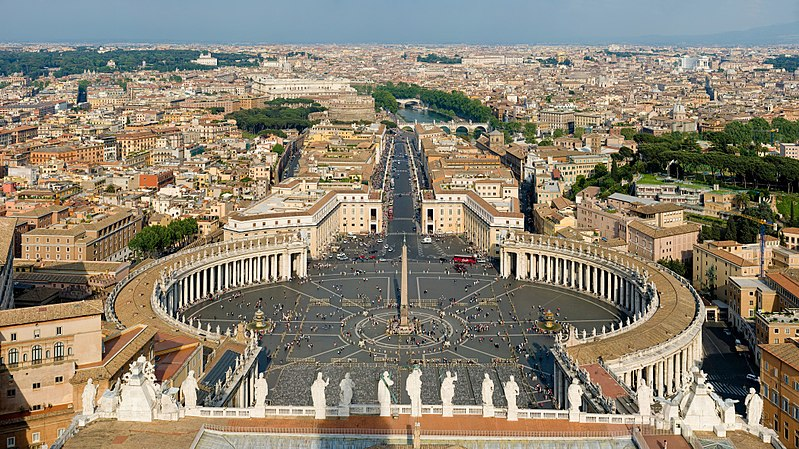
\includegraphics[width=1.00\linewidth]{../images/800px-St_Peter's_Square,_Vatican_City_-_April_2007}
	\caption{St Peter's Square, Vatican City - April 2007. {\footnotesize (Photo by David Iliff. License: CC-BY-SA 3.0 \ccbysa. Courtesy of \href{https://upload.wikimedia.org/wikipedia/commons/d/d6/St_Peter\%27s_Square\%2C_Vatican_City_-_April_2007.jpg}{ Wikimedia Commons}.)}}
	\label{fig:640px-stpeterssquarevaticancity-april2007}
\end{figure}
		
	\subsection{Latin lyrics by \hyperref[ref4]{Lavagna (1991)}\label{ref4-d}}
		\label{latin-lyrics-by-lavagna-1991}
		
	{
	\fboxsep 0pt % default: 3pt
	\fboxrule 0.2pt % default: 0.4pt
	\begin{figure}
	\centering
	\fbox{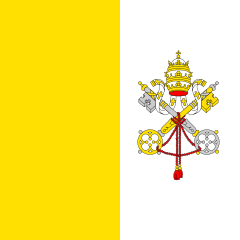
\includegraphics[width=0.20\linewidth]{../images/240px-Flag_of_the_Vatican_City-svg}}
	\caption{Flag of the Vatican City. {\footnotesize (Author unknown. License: Public Domain \ccPublicDomain\ccZero. Courtesy of \href{https://upload.wikimedia.org/wikipedia/commons/0/00/Flag_of_the_Vatican_City.svg}{Wikimedia Commons})} }
	\label{fig:240px-flagofthevaticancity}
	\end{figure}}

	
\begin{minipage}{3.0in}
	\begin{description}
		%\tightlist
		\item[]
		\textbf{Original Latin}%\footnote{}\\
		\hspace*{0.333em}

			
		\begin{description}
			%\tightlist
			\item[]
			CHORUS
		\end{description}
		
		O felix Roma, O felix Roma nobilis.
		
		O felix Roma, Roma felix Roma nobilis.
		
		Sedes es Petri, qui Christi vicem gerit,
		
		Sedes es Petri, qui apostolus est pacis.
		
		${}_{}$
		
		${}_{}$
	\end{description}

	\begin{description}
		%\tightlist
		\item[]
		
		Pontifex tecum erimus omnes nos
		
		Pontifex es magister qui tuos confirmas fratres.
		
		Pontifex tecum erimus omnes nos
		
		Pontifex es magister qui tuos confirmas fratres.
		
		Pontifex fundamentum ac robur nostrum,
		
		Hominumque piscator pastor es gregis ligans terram et coelum.
		
		${}_{}$
	\end{description}
	
	\begin{description}
		%\tightlist
		\item[]
		Petre, tu es Christi es Vicarius super terram,
		
		Rupes inter fluctus, tu es pharus ac veritas.
		
		Tu Christi es caritas, tu es unitatis custos,
		
		Promptus libertatis defensor; in te auctoritas.
		
		Petre, tu es Christi es Vicarius super terram,
		
		Rupes inter fluctus, tu es pharus ac veritas.
		
		Tu Christi es caritas, tu es unitatis custos,
		
		Promptus libertatis defensor; in te auctoritas.
			
		${}_{}$
		
		${}_{}$
	\end{description}
\end{minipage}	
\hspace{0.15in}
\begin{minipage}{3.0in}
	\begin{description}
		%\tightlist
		\item[]
		\textbf{An English translation}
		
		\begin{description}
			%\tightlist
			\item[]
			CHOIR
		\end{description}
		
		O happy Rome , O happy Rome, the most famous.
		
		O happy Rome, Roma felix noble Rome.
		
		You are the seat of Peter, who takes the place of Christ,
		
		You are the seat of Peter, who is an apostle of peace.
\end{description}
	

	\begin{description}
		%\tightlist
		\item[]
		Pope will be with us all
		
		Are the teacher of the Pope who, you confirm your brethren.
	
		Pope will be with us all
	
		Are the teacher of the Pope who, you confirm your brethren.
		
		And the strength of the foundation of our high priest,
		
		The shepherd of the flock, linking heaven and earth and fisher of men.
	\end{description}
	
	\begin{description}
		%\tightlist
		\item[]
		Peter, you are the vicar of Christ on the earth,
		
		Amidst the waves, you are a beacon, and the truth.
		
		You are the love, you are the guardian of unity,
		
		Prompt defender of liberty; authority in you.
		
		Peter, you are the vicar of Christ on the earth,
		
		Amidst the waves, you are a beacon, and the truth.
		
		You are the love, you are the guardian of unity,
		
		Prompt defender of liberty; authority in you. 
	\end{description}
\end{minipage}
	
	\subsection{See also}\label{see-also}
	
	\begin{itemize}
		%\tightlist
		\item \href{https://en.wikipedia.org/wiki/Index_of_Vatican_City-related_articles}{Index of Vatican City-related articles}
	\end{itemize}
	
	\subsection{References}\label{references}
	\begin{itemize}
		\item[] [1]\label{ref1}\textasciicircum$^{\hyperref[ref1-a]{a}, \hyperref[ref1-b]{b}, \hyperref[ref1-c]{c}, \hyperref[ref1-d]{d} }$
		\href{http://www.vaticanstate.va/content/vaticanstate/en/stato-e-governo/note-generali/inno.html}{Pontifical Anthem and its History.}  From the official site of Vatican City State. Accessed on 2017-09-17.
		
		\item[] [2]\label{ref2}\textasciicircum$^{\hyperlink{ref2-a}{a}, \hyperlink{ref2-b}{b}}$ \href{http://www.vatican.va/news_services/press/documentazione/documents/sp_ss_scv/inno/inno_scv_storico_it.html}{Pontifical Anthem and its History} (in Italian).  From the official site of Vatican City State. Accessed on 2017-09-17.
		
		\item[] [3]\label{ref3}\textasciicircum$^{\hyperref[ref3-a]{a}, \hyperref[ref3-b]{b}}$
		\href{http://www.vatican.va/news_services/press/documentazione/documents/sp_ss_scv/inno/inno_scv_partitura_coro_indice_it.html}{Score for choir of four voices by Alberico Vitalini with original Latin text by Monsignor Raffaello Lavagna.} From the official site of the Holy See. Accessed on 2017-09-17.
		
		\item[] [4]\label{ref4}\textasciicircum$^{\hyperref[ref4-a]{a}, \hyperref[ref4-b]{b}, \hyperref[ref4-c]{c}, \hyperref[ref4-d]{d} }$
		\href{http://www.vatican.va/news_services/press/documentazione/documents/sp_ss_scv/inno/inno_scv_testo_it.html}{Inno Pontificio} lyrics, with brief historical notes and MIDI file. From the official site of the Holy See. Accessed on 2017-09-17.
	\end{itemize}


	\subsection{Media}\label{media}
		\href{https://upload.wikimedia.org/wikipedia/commons/8/8d/Pontifical\_March.pdf}{PDF}, info
		\href{https://en.wikipedia.org/wiki/File:Pontifical\_March.pdf}{here}

	\subsection{External links}\label{external-links}
	\begin{itemize}
		%\tightlist
		\item
		\href{http://www.vaticanstate.va/EN/State_and_Government/General_informations/Anthem.htm}{Official
			site of Vatican City State}
		\item
		\href{http://nationalanthems.me/vatican-city-holy-see-marche-pontificale}{Streaming
			audio, lyrics and information about the Pontifical Anthem}
	\end{itemize}

	\subsection{License \ccbysa}
	This work, \textit{Marche Pontificale}, by J.L.A. Uro includes text from the {\tt Wikipedia:~Pontifical~Anthem} article and, as the text of that article, is distributed under the \href{https://creativecommons.org/licenses/by-sa/3.0/}{Creative Commons Attribution-ShareAlike 3.0 Unported License}.
	
	\subsection{Acknowledgments}
 Special thanks to the \href{http://imslp.org/}{International Music Score Library Project (IMSLP)} for making available the the public domain scores for \href{http://ks.imslp.net/files/imglnks/usimg/6/60/IMSLP258526-PMLP114725-Gounod_-_Marche_pontificale_ArrPf.pdf}{\em Marche Pontificale (1870)} and \href{http://hz.imslp.info/files/imglnks/usimg/e/e8/IMSLP55496-PMLP114725-Gounod,_Ch._Marche_Pontificale.pdf}{\em Marche Pontificale (1924)}.  My sincerest gratitude to Chris Walshaw et al.\ for the \href{http://www.abcnotation.com/}{ABC music notation}; Jean-Francois Moine for \href{http://moinejf.free.fr/}{\tt abcm2ps}; Guido Gonzato for the \href{http://abcplus.sourceforge.net/}{ABC Plus Project} and the \href{http://abcplus.sourceforge.net/#abcMIDI}{{\tt abcmidi} resources} available there, more especially for the ABC resource book {\em Making Music with ABC 2}; James R. Allwright and Seymour Shlien for \href{http://abc.sourceforge.net/abcMIDI}{\tt abcmidi} source and binaries; Nils Liberg for \href{http://www.nilsliberg.se/ksp/easyabc/}{EasyABC}; John MacFarlane for \href{http://pandoc.org}{\tt pandoc} (used for converting {\tt mediawiki} to {\tt latex});  \href{https://artifex.com/}{Artifex, Inc.} for Ghostscript v.9.06 (includes the {\tt ps2pdf} converter);  \href{https://www.inkscape.org/}{Inkscape v.0.48.5} for the tool for converting SVGs to PDFs for inclusion into \LaTeX\ documents; and \href{https://tex.stackexchange.com/users/632/martin-h}{\tt User:Martin H} for his \href{https://tex.stackexchange.com/questions/2099/how-to-include-svg-diagrams-in-latex}{reply} to a TeX/LaTeX Stack Exchange question on including SVGs into \LaTeX\ documents.  Many thanks, too, to the \href{https://www.debian.org}{Debian Project} for the Debian 8 (Jessie) GNU/Linux OS, \href{http://www.tug.org/texlive/}{TeXLive} for providing the \TeX\ distribution,  and \href{https://github.org}{GitHub} for its generosity in providing space for \href{https://github.com/justineuro/MP}{the project}.
	
\section{Musical Score: {\em Marche Pontificale (1869)}}
	As most of the versions of the {\em Marche Pontificale} mentioned above are currently still copyrighted, the musical score that follows is from two musical scores (\href{http://ks.imslp.net/files/imglnks/usimg/6/60/IMSLP258526-PMLP114725-Gounod_-_Marche_pontificale_ArrPf.pdf}{\em Marche Pontificale (1870)} and \href{http://hz.imslp.info/files/imglnks/usimg/e/e8/IMSLP55496-PMLP114725-Gounod,_Ch._Marche_Pontificale.pdf}{\em Marche Pontificale (1924)}) that were obtained from the \href{http://imslp.org}{International Music Score Library Project (IMSLP)}.  These two (2) arrangements were based on the original 1869 work of Charles Gounoud. 

\newpage
${}_{}$\vspace{0.25in}
{\centering

	\begin{figure}[H]
		\centering
		\def\svgwidth{\columnwidth}
		\input{MP001.pdf_tex}
	\end{figure}

\newpage
${}_{}$\vspace{0.25in}
	\begin{figure}[H]
		\centering
		\def\svgwidth{\columnwidth}
		\input{MP002.pdf_tex}
	\end{figure}
}	
\nopagebreak[4]{For audio (midi): \href{https://justineuro.github.io/MP/MarchePontificale.mid}{MarchePontificale.mid}} 	
\end{document}